\documentclass[tikz,border=6pt]{standalone}
\usepackage{amsmath}
\usepackage{bm}
\usetikzlibrary{arrows.meta,decorations.markings,calc}

\begin{document}
	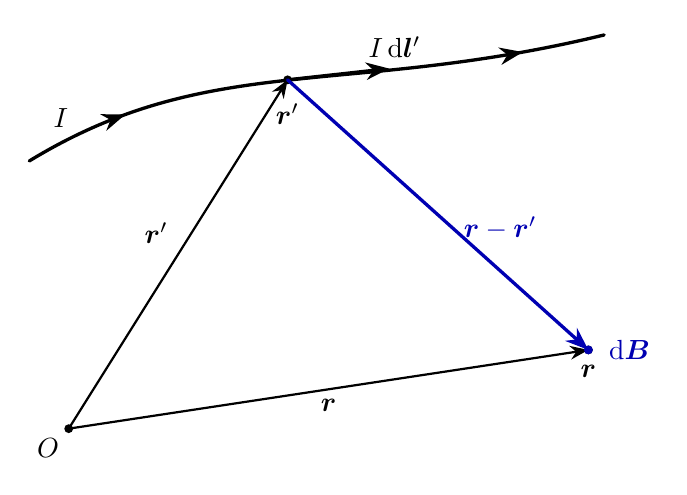
\begin{tikzpicture}[>=Stealth,line cap=round]
		
		% ---- 原点 ----
		\coordinate (O) at (0,0);
		\fill (O) circle (1.6pt) node[below left] {$O$};
		
		% ---- 载流细导线（更长的三次贝塞尔）----
		% 控制点: P0(-0.5,3.4) P1(1.8,4.8) P2(3.5,4.2) P3(6.8,5.0)
		\draw[very thick,
		postaction={decorate},
		decoration={markings,
			mark=at position 0.18 with {\arrow{Stealth}},
			mark=at position 0.86 with {\arrow{Stealth}}}]
		(-0.5,3.4) .. controls (1.8,4.8) and (3.5,4.2) .. (6.8,5.0);
		\node at (-0.1,3.95) {$I$};
		
		% ---- 源点 r' = B(0.5) = (2.78,4.43) ----
		\coordinate (S) at (2.78,4.43);
		\fill (S) circle (1.6pt);
		\node[below] at ([yshift=-5pt]S) {$\bm{r}'$};
		
		% ---- 电流元 I dl'：严格沿 t=0.5 处切向 (0.994,0.110) ----
		\draw[->,very thick,black]
		(S) -- ++(1.29,0.143)
		node[above,xshift=2pt] {$I\,\mathrm{d}\bm{l}'$};
		
		% ---- 场点 r ----
		\coordinate (P) at (6.6,1.0);
		\fill (P) circle (1.6pt);
		\node[below] at ([yshift=-2pt]P) {$\bm{r}$};
		
		% ---- 位置矢量 r' 和 r ----
		\draw[->,thick] (O) -- (S) node[midway,above left] {$\bm{r}'$};
		\draw[->,thick] (O) -- (P) node[midway,below] {$\bm{r}$};
		
		% ---- 间隔矢量 (r - r')，点缀色 ----
		\draw[->,very thick,blue!70!black]
		(S) -- (P)
		node[pos=0.55,right] {$\bm{r}-\bm{r}'$};
		
		% ---- dB 垂直纸面（纸外），放在矢量末端（场点）处 ----
		
		\fill[blue!70!black] (P) circle (1.6pt);
		\node[blue!70!black,right] at ([xshift=4pt]P) {$\mathrm{d}\bm{B}$};
		
	\end{tikzpicture}
\end{document}